\section{Best-Selling Albums Dataset}

{\bf Attributes:} Year, Ranking, Artist, Album, Genre, Worldwide Sales, Tracks, Album Length\\

{\bf Scenario:} A media analytics firm is interested in understanding whether certain genres consistently produce top-selling albums or if success is more scattered across genres.\\

{\bf Research Question:} How does the distribution of album sales vary across music genres for albums in the previous decade (released after 2015), and are high-sales outliers concentrated in certain genres?

\subsection{Part A: Data Cleaning and Preprocessing}
First, filter your dataset so that only the variables critical for your analysis remain. Then clean your data so that there is consistency in variable types, capitalization, and handle any missing or invalid values.\\
-----\\
The album data set had multiple issues that needed to be addressed. First, we pre-processed the data points by thresholding them based on their 'Year' attribute to include only those released after 2015 because that is the window of interest to this hypothetical firm. Then we removed the features not critical to the analysis of album sales by genre, leaving only 'Worldwide Sales (Est.)' and 'Genre'. On that note, we standardized the column names under snake case as 'album\_sales' and 'genres', respectively.\\

In terms of cleaning the attribute values themselves, we standardized the casing of the genre values and then checked this step by printing a dictionary of genres as keys, mapped to their respective counts. Before this casing step was enforced, printing the dictionary revealed that one genre value was written as "HIp Hop" and had defined two separate keys for the one genre.\\

The final cleaning step expresses each of the album sale values as an integer data type without any commas so that they would not be conflated as delimiters in the CSV file.\\

We wrote this utility function to accomplish the task:

\begin{verbatim}
def clean_preprocess_albums_data(input_csv: str, output_csv: str) -> pd.DataFrame:
    """
    Cleans and preprocesses the albums dataset by removing irrelevant
    features and data points, handling missing/invalid values, standardizing
    capitalization, and converting data types. 

    :param input_csv:: Path to the input CSV file containing the albums dataset.
    :type input_csv: str
    :param output_csv: Filename for the clean data.
    :type output_csv: str
    :returns: pd.DataFrame
    :rtype: pd.DataFrame
    """
    df = pd.read_csv(input_csv)

    # Keeps critical variables, relevant data points, removes missing value rows,
    # and renames columns more appropriately
    df = df[df['Year'] > 2015]
    df = df.iloc[:, [4, 7]]
    df.dropna(inplace=True)
    df.columns = ['album_sales', 'genre']

    # Confirms there aren't duplicate genres due to misspelling/invalid vals
    # and standardizes capitalization
    df['genre'] = df['genre'].str.lower()
    print(df['genre'].value_counts().to_dict())

    # Reformats albums sales as integers
    df['album_sales'] = df['album_sales'].str.replace(',', '').astype(int)

    os.makedirs(os.path.dirname(f'../datasets/clean/{output_csv}'), exist_ok=True)
    df.to_csv(f'../datasets/clean/{output_csv}', index=False)
    return df
\end{verbatim}

\begin{center}
\textbf{Figure 1:} Best-Selling Albums data pre-processing function.
\end{center}

Below is a comparison of the head of each version to illustrate the changes that were made:\\

\noindent\textbf{Top\_10\_Albums\_By\_Year.csv}
\begin{verbatim}
Year,Ranking,Artist,Album,Worldwide Sales (Est.),Tracks,Album Length,Genre
1990,1,Madonna,The Immaculate Collection,"30,000,000",17,73:32,Pop
1990,2,New Kids On The Block,Step By Step,"20,000,000",12,47:44,Pop
1990,3,Garth Brooks,No Fences,"18,770,000",10,34:34,Country
1990,4,MC Hammer,Please Hammer Don't Hurt Em,"18,000,000",13,59:04,Hip Hop
1990,5,Mariah Carey,Mariah Carey,"15,000,000",11,46:44,Pop
1990,6,Movie Soundtrack,Aashiqui,"15,000,000",12,58:13,World
1990,7,Whitney Houston,I'm Your Baby Tonight,"10,000,000",11,53:45,Pop
1990,8,Phil Collins,Serious Hits... Live!,"9,956,520",15,76:53,Rock
1990,9,Enigma,MCMXC A.D.,"8,838,000",7,40:16,Pop
1990,10,The Three Tenors,Carreras Domingo Pavarotti In Concert 1990,"8,533,000",17,67:55,Classical
...
\end{verbatim}

\noindent\textbf{album\_sales\_by\_genre.csv}
\begin{verbatim}
album_sales,genre
7657000,hip hop
6111355,hip hop
4421666,r&b
4207235,pop
4170954,pop
3661560,pop
3462374,pop
3418440,pop
3189149,pop
2727078,pop
...
\end{verbatim}

\begin{center}
    \textbf{Figure 2:} Raw vs. Cleaned Best-Selling Albums dataset.
\end{center}
\newpage

\subsection{Part B: Generate Three Visualizations}
Produce the following types of plots:
\begin{itemize}
    \item \textbf{Error Bar Plot:} Show the mean and variability (e.g., standard error or 95\% confidence intervals) of the numerical variable across each category.
    \item \textbf{Barcode Chart:} Also known as a strip plot or rug plot. Shows individual data points across categories.
    \item \textbf{Histogram:} Plot the distribution of the numerical variable, grouped by the categorical variable (using hue or facet).
\end{itemize}
-----\\
\textbf{Error Bar Plot}
\begin{center}
  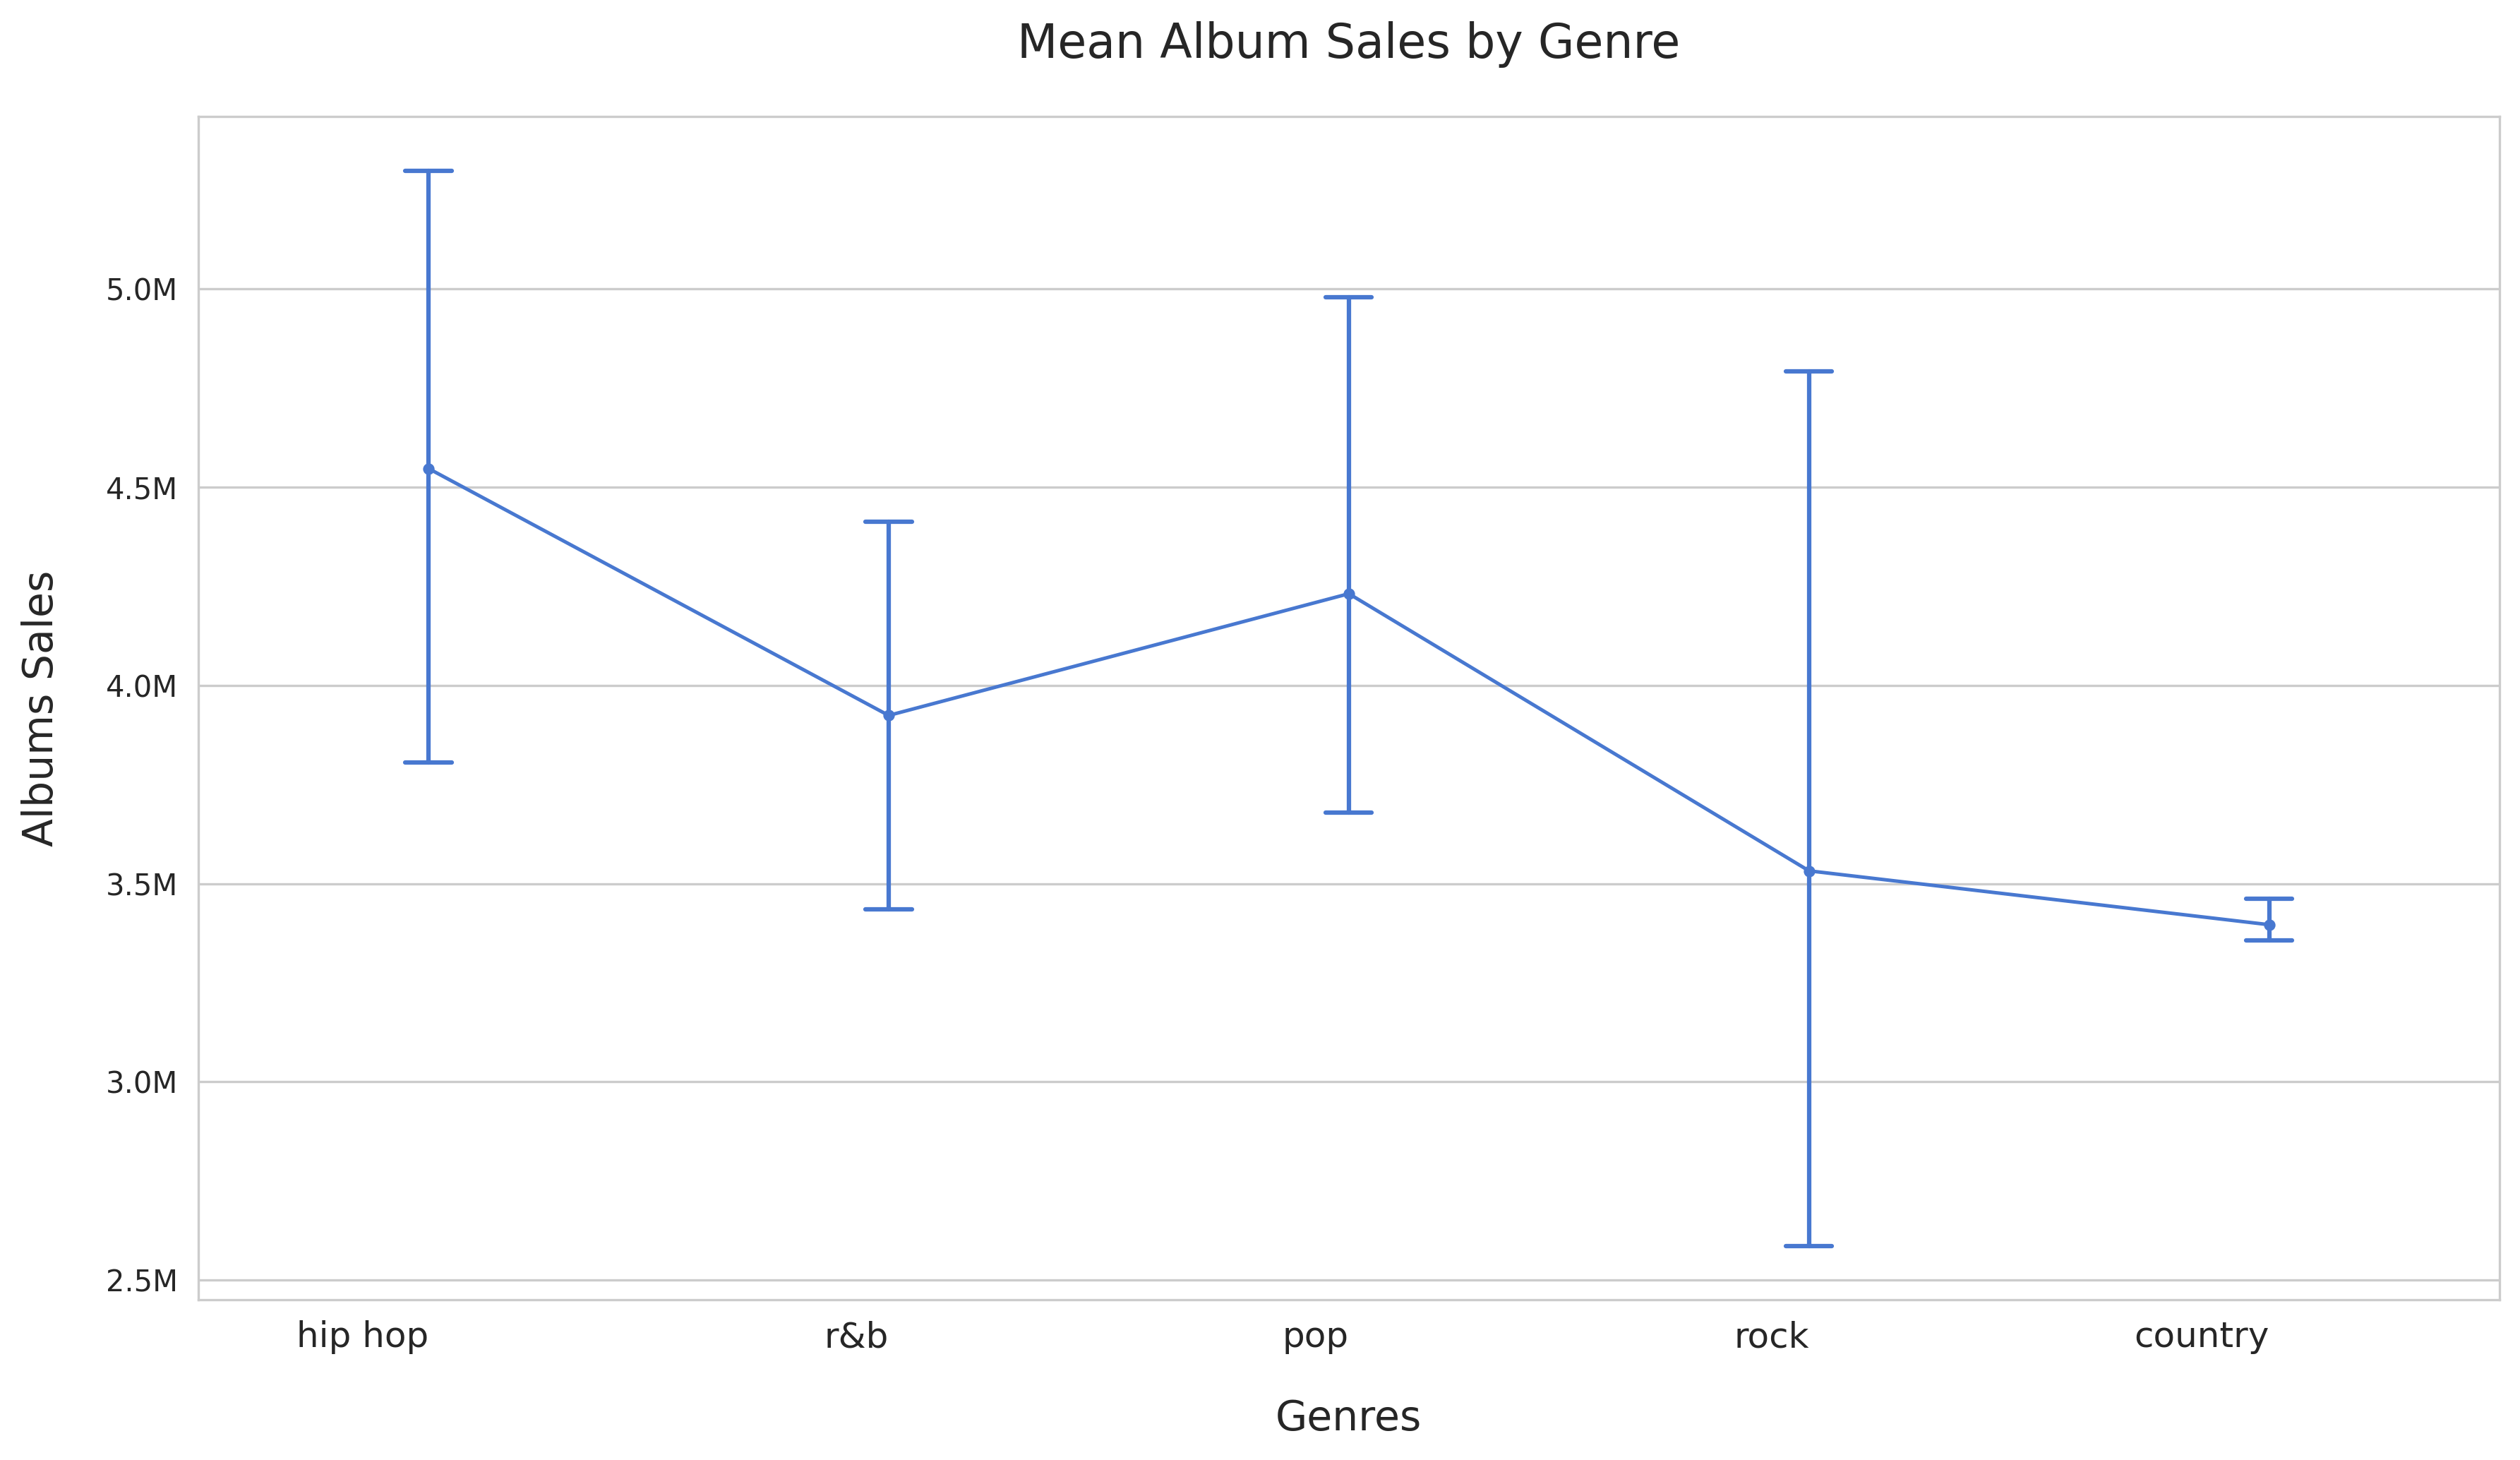
\includegraphics[width=0.95\textwidth]{figures/album_sales_by_genre_error_bar_plot.png}
  
  \textbf{Figure 3:} Mean Album Sales by Genre with 95\% confidence intervals.
\end{center}

\textbf{Barcode Chart}
\begin{center}
  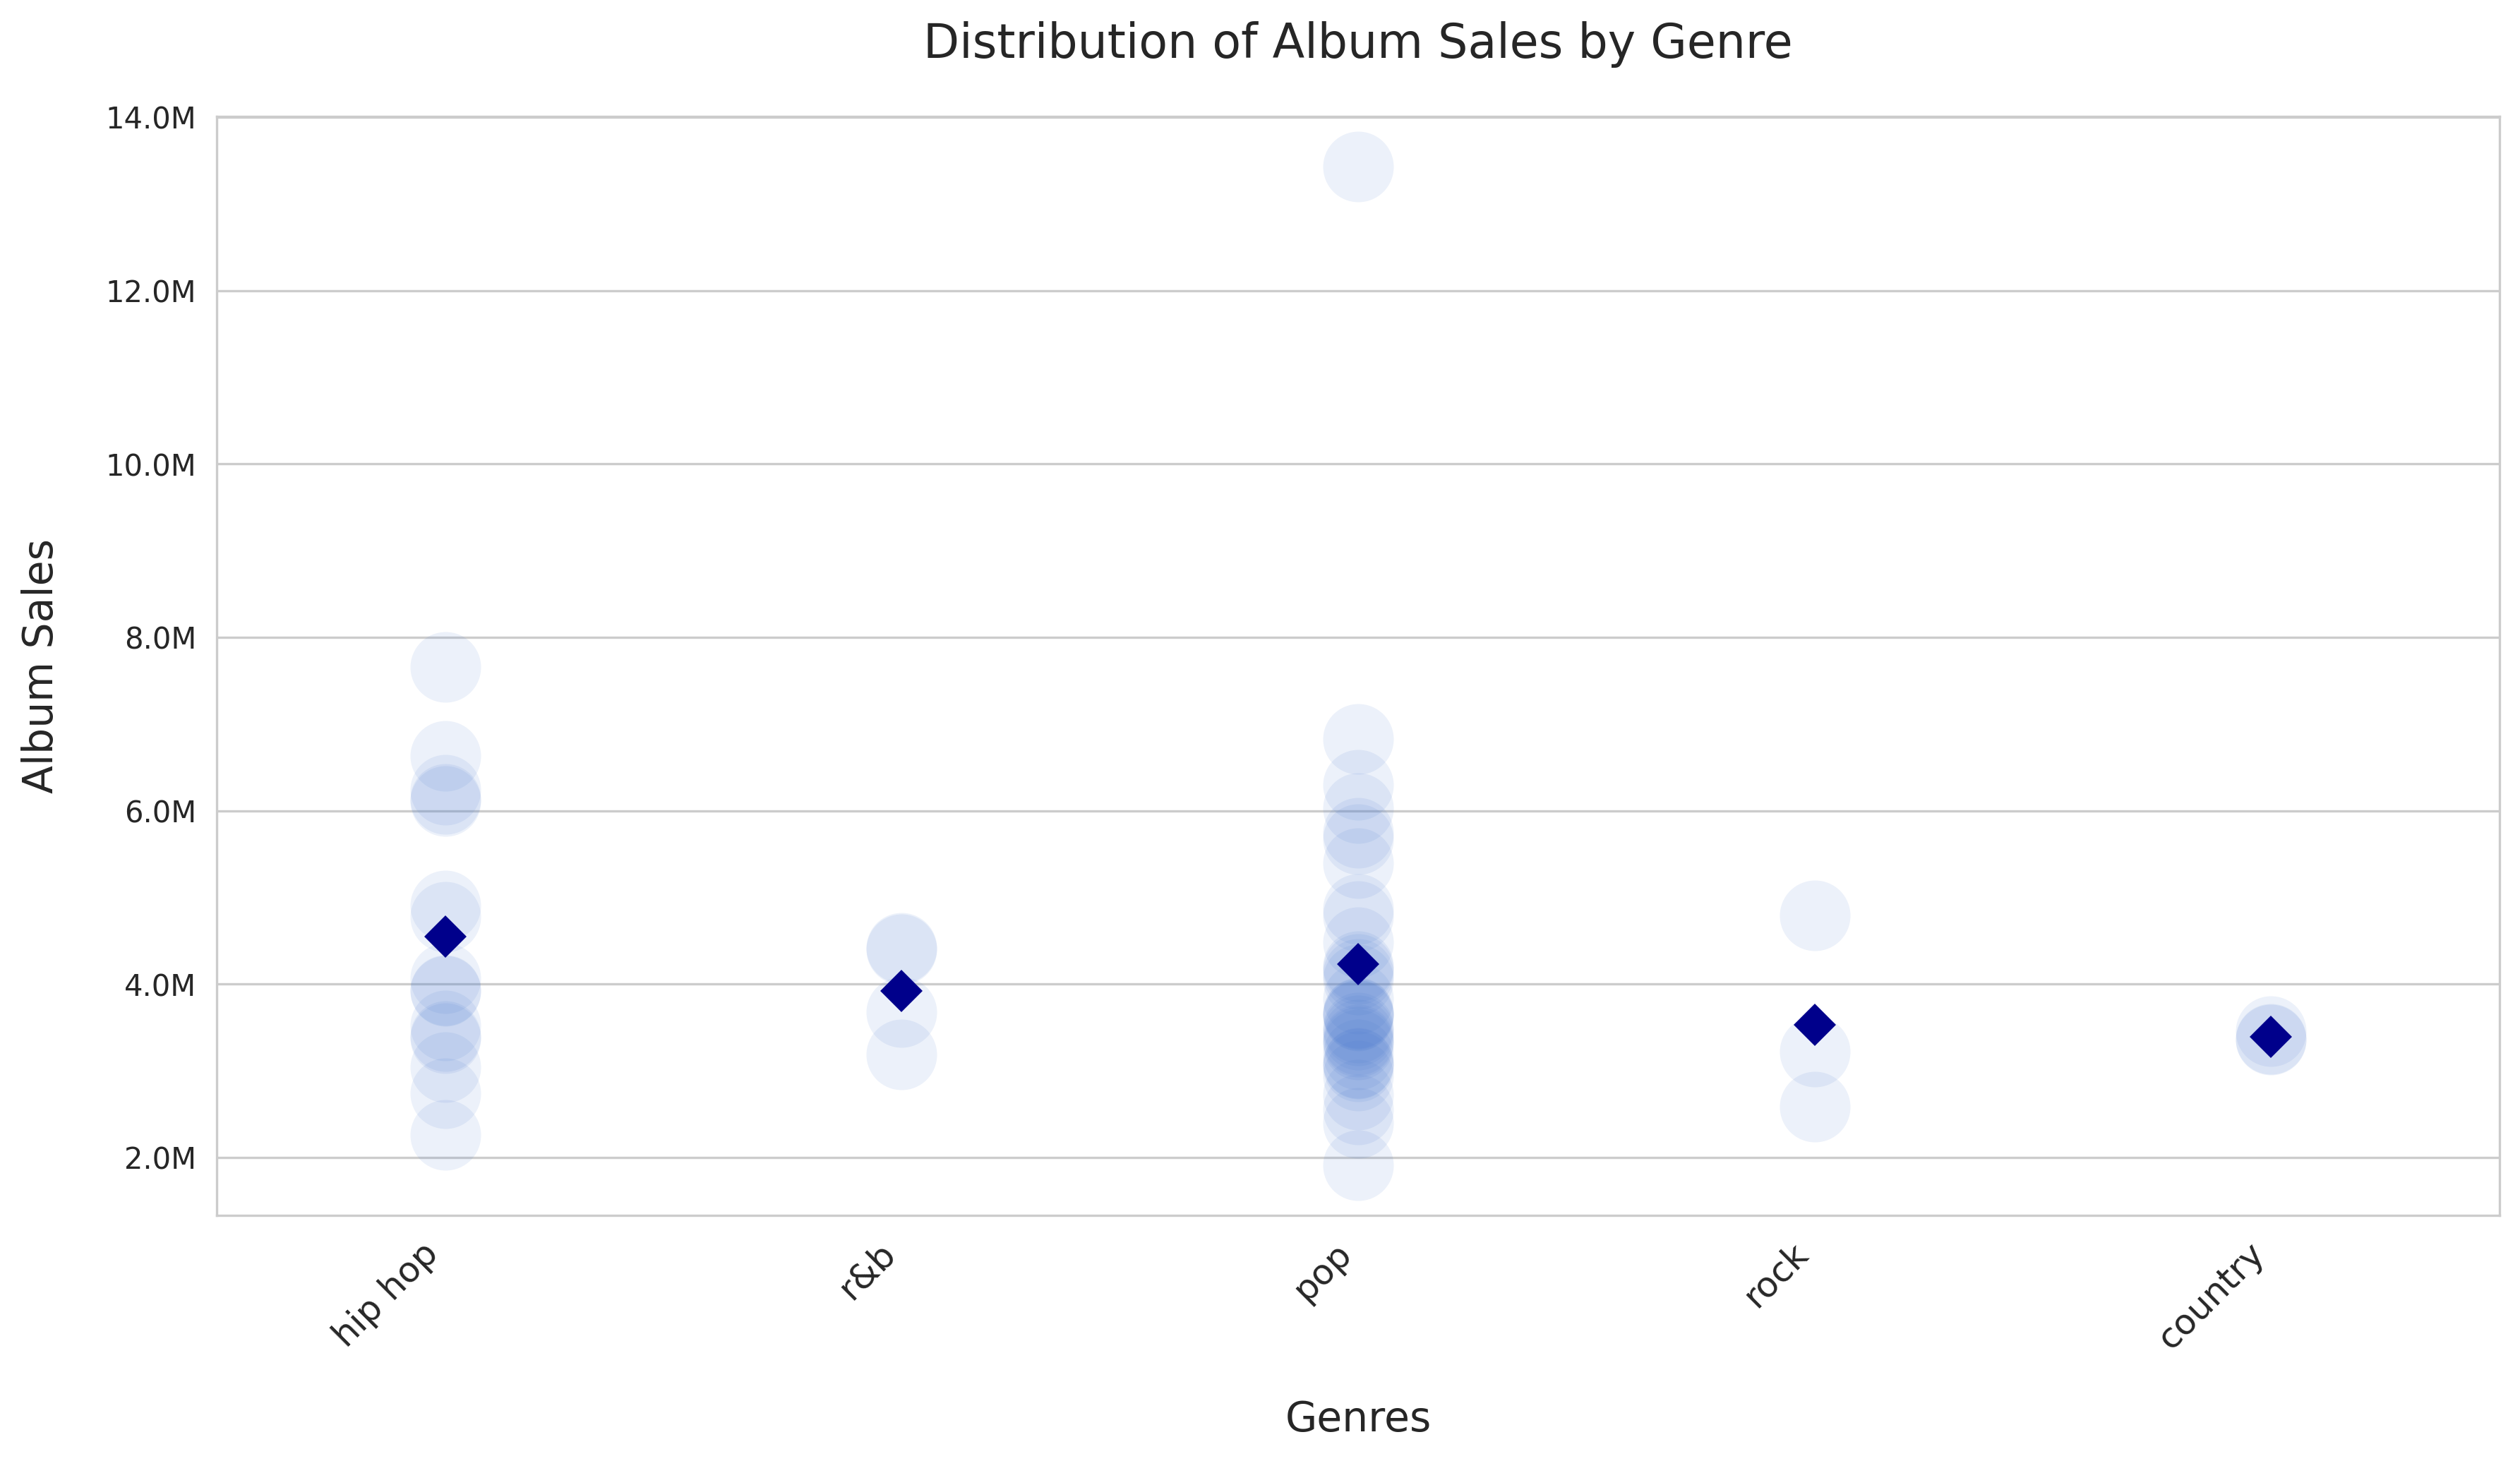
\includegraphics[width=0.95\textwidth]{figures/album_sales_by_genre_strip_plot.png}
  
  \textbf{Figure 4:} Average Distribution of Album Sales by Genre.
\end{center}

\textbf{Histogram}
\begin{center}
  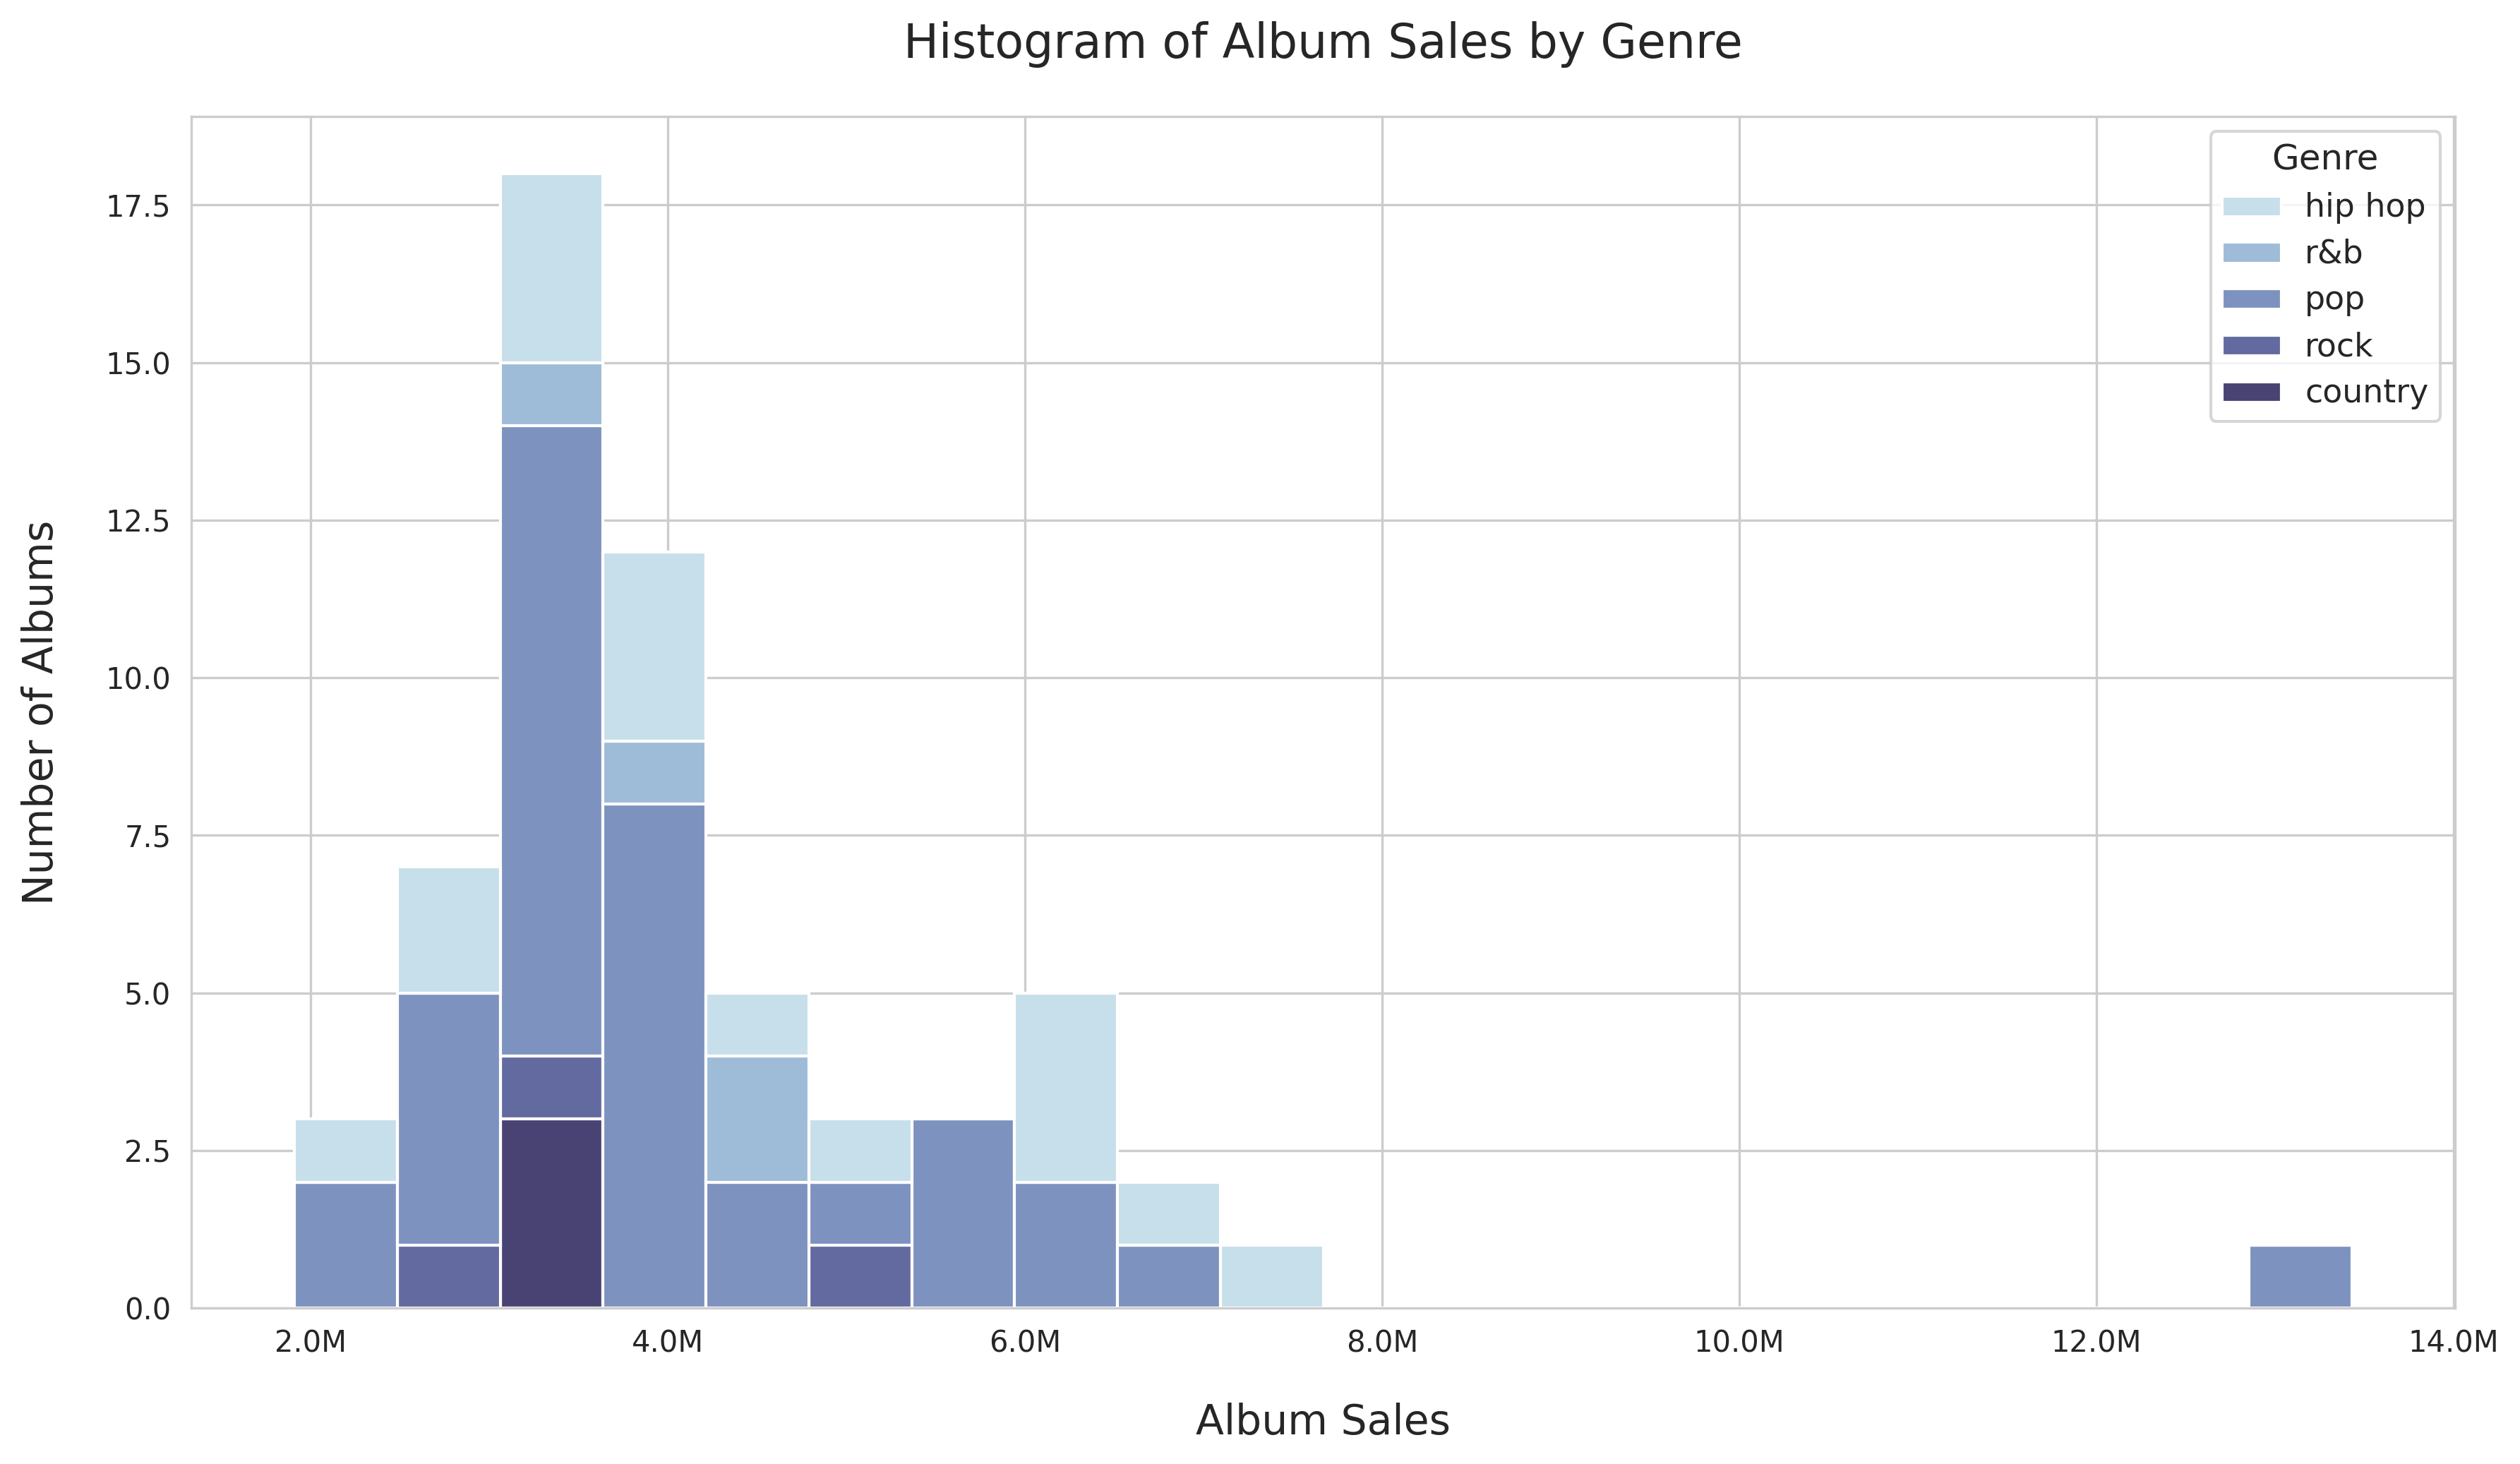
\includegraphics[width=0.95\textwidth]{figures/album_sales_by_genre_histogram_plot.png}
  
  \textbf{Figure 5:} Histogram of Album Sales by Genre.
\end{center}

\subsection{Part C: Evaluate and Justify Visualization}
For the dataset:
\begin{itemize}
    \item Discuss the advantages and disadvantages of each visualization type.
    \item Decide which visualization is best for the research question.
    \item Support your answer with evidence from the plots and reasoning based on dataset size, shape, or structure.
\end{itemize}
-----\\
\textbf{Advantages and Disadvantages}\\

The error bar plot well-represents the spread of the data out to our specific confidence level, giving us a notion of uncertainty in this understanding of the distributions, and shows clearly the average number of album sales for each genre. Where the error bar plot loses out, however, is in their ability to represent outliers/non-general cases out to our uncertainty threshold. This plot gives us no knowledge of what the distribution looks like outside the error bars, and within the error bars, we do not get to see the shape that the distribution's mass forms directly, it only signals this shape by the information we can gather from the mean points and the error bar lengths. We can also see in later visualizations that the mass distribution for each genre does look a bit different and so there is some necessary context getting lost for this data. Additionally, while the notion of uncertainty in understanding variance is informative, it is not as useful for the genres where data is very sparse, and so in the cases of genres like Rock or Country, the understanding of their variance in this plot could very well be over- or under- exaggerated.\\

The strip plot does a great job at contending with the spread of the data; as we saw in class, the density of the points is a very natural indicator of how the mass of the distribution is laid out across its domain, and we also get on top of that direct knowledge of what outliers exist for each genre and what that behavior looks like comparatively for each genre. We can see from the figure one relatively extreme outlier in the Pop genre that was not obvious before with the error bar plot; an Ed Sheeran album called "Divide" from 2017, achieving just north of 13.4 million sales. This plot also tends to include a mean indicator, which we have included as a distinct, opaque symbol overtop the data points, and this is very helpful in understanding the difference between the extreme behavior and the typical behavior for each genre. The sole issue we have with this visualization is that it is still one step/"layer" away from getting the full benefit of viewing a distribution plotted for each genre directly. Nevertheless, for this particular context, we are examining a fairly small number of examples (only releases after 2015), so any issues with too much overlap and a lack of clarity in how the mass is distributed is not something that we will struggle with much here.\\

The histogram is primarily helpful in the exact area where the strip plot can fail, where perhaps the mass of the distribution is hard to interpret due to this overlapping quality of its visuals and perhaps we could be looking at a larger set of samples in some cases, and so here we get the benefit of most directly viewing how the mass is distributed over the different bins of album sales for each genre. Regarding each genre though, one concern we have is that, regardless of every color palette we tried, reading the behavior of each distribution comparatively i.e. between genres is obfuscated by the fact that they are all plotted on the same figure and the shapes of these distributions are not as smooth because of how few samples we are analyzing. Where we benefit much more with histograms is in examining the extreme values and in understanding the general tendencies of the data. Again, we would argue that strip plots represent these behaviors better for this data, but nonetheless histograms do well to provide us with this context, certainly well enough to make informed claims about the samples. The sole struggle here is just with comparing the genres as effectively.\\

\textbf{Which visualization is best for the research question}\\

How does the distribution of album sales vary across music genres for albums in the previous decade (released after 2015), and are high-sales outliers concentrated in certain genres? The strip plot is best for answering this research question.\\

\textbf{Evidence-based Support for this answer}\\

First, let's compare the information we collect from the error bar plot versus the strip plot. Both give us very clearly the mean values for each genre, so when contending with the question of album sales varying across genres, we can equally speak to the general behavior of each genre. Both tell us that Hip-Hop and Pop sells the most albums on average, having a noticeably higher mean, followed by R\&B and Rock, and trailed by Country with a noticeably lower average sale performance. We will concede though that the error bar plot does do marginally better to comparatively visualize the mean values across genres due to the fact that it does not have to scale to extreme outliers in the data, allowing it to be more expressive in this respect. Nonetheless, one can still look at the strip plot and immediately make the comparisons we just did, it is just not as obvious.\\

Regrading the variance of the data, the strip plot gives us information more relevant to our research question, as we are concerned with high-sales outliers in our data. It is obvious from the shape of our data for each genre that the error bar plot completely misses the primary point to take away from the data in this respect; that being the high-sale outlier in the Pop genre. The strip plot makes it immediately clear and is the obvious choice as far as understanding the whole second part of our research question. Additionally, the error bars, while informative in the case of genres with a lot of exposure in the top 10 over the past decade, struggle to provide as much leverage to make claims about the general behavior of sparser genres. Again, as the strip plot provide a much more direct visualization of how the data is distributed, it is the obvious choice over error bar plot for answering the research question. \\

As far as choosing between the strip plot and the histogram, we confirmed in class and previously from the discussion of advantages and disadvantages that the strip plot mainly loses value in the cases that there is so much data, or perhaps the data is so concentrated toward the distribution's center, that it could be hard to understand the variance for each genre. That is not the case here and the strip plot actually does quite a good job at representing the relative spread in the data across genres; in this case, it's like staring at the distributions from a bird's-eye view, uninhibited by any overlapping masses across genres and expressive enough to readily show qualities like the extra mass of the left side of the pop genre distribution of album sales and the relative difference in variance between rock, pop, and hip hop.
\newpage